\chapter{Publication bias}
\label{chap:four}
% grammar checked (07-27)

\begin{quoting}
\textit{An investment in knowledge pays the best interest.}
\end{quoting}
\vspace{-0.2em}
\hfill --- Benjamin Franklin
\vspace{0.5em}

It is widely acknowledged that attending school brings numerous benefits for one's future. To claim the opposite would simply appear foolish, considering the vast quantities of existing literature that explore the positive impact of schooling \citep{oreopoulos2013making, ritchie2018much, heckman2010rate, psacharopoulos2004returns}. However, what happens if a researcher conducts an experiment, and the results suggest that education hurts the prospects of the subjects that took part? Such an experiment will most likely be viewed skeptically, if not frowned upon. The initial response of the publishers presented with such results might, in most cases, go more along the lines of "Perhaps there is something wrong with your setup?" rather than "Truly, what a revolutionary discovery!" In expectation of such a response and considering the time and often money invested into the experiment, the researcher is posed with a tough decision - keep the results as is, or sacrifice legitimacy in return for better publication prospects?

The issue described above is commonly referred to as publication bias and is exactly what this part of the paper explores. Among the many forms this malpractice can take, perhaps two are the most prominent. Firstly, studies can remain unpublished due to the discrepancy between their results and the existing knowledge, also known as the \textit{file drawer problem} \citep{stanley2005beyond}. Secondly, the results within those studies may be modified to gain higher order of statistical significance; this can be done by modifying the standard error or even the effect itself - a form of malpractice sometimes referred to as p-hacking \citep{simmons2011false}. Luckily, this manipulation can be detected within the data using various statistical tests, given the unnatural patterns that the p-value distribution tends to exhibit in case such practices are employed.

Regarding publication bias in the literature on returns to education, five of the ten existing meta-analyses address the issue, as mentioned in \autoref{chap:two}. Out of these five studies, three detect the presence of publication bias, while two do not. These conflicting results leave a lot to be desired. For this, I find it crucial to shed more light on the publication bias issue and hope to bring further vital evidence.

In the rest of this chapter, I will first graphically explore the relationship between the effect and the standard effect using a simple visual test. Next, I will conduct multiple linear and non-linear tests to determine whether a quantifiable link exists between the two variables. I will also employ methods that do not assume any prior form of the relationship and test for structural breaks in the distribution of t-statistics in the data. Lastly, I will bring three completely new methods into the picture. These should help me detect p-hacking in the data and link the results together across multiple models with means of model averaging.

\section{Funnel Plot}
\label{sec:funnel_plot}

I first test for publication bias using the funnel plot \citep{Egger1997, stanley2005beyond}. The genius of the method lies in its simplicity, where the main effect is plotted on the x-axis against a measure of precision on the y-axis. Usually (and in this case, too), the precision is calculated simply as the inverse of the standard error. Although \cite{stanley2005beyond} suggests that alternatives can be used, such as the square root of the degrees of freedom, I opt for the standard error. After the plot is constructed, the most precise estimates should be clustered around the true effect mean, assuming that the data contains no publication bias, systematic heterogeneity, or small-sample effects. As precision decreases, the estimates get more scattered, creating an inverted funnel shape. In this shape, gaps or holes hint that data tampering exists within the literature.

As mentioned above, I construct the funnel plot using the inverted standard error as the measure for precision because all estimates in the dataset have their standard error reported (this was one of the conditions during data collection, as described in \autoref{chap:three}). Apart from a funnel plot with all collected data points, I also present a figure that displays only the medians of the effect for all 74 studies. These two graphs appear in the sub-figures of \autoref{fig:funnel_plot}.

\begin{figure}[!t]
\begin{center}
\caption{The funnel plot shows no immediately suspicious patterns}
\label{fig:funnel_plot}
\begin{subfigure}[b]{0.45\textwidth}
   \caption{All observations}
   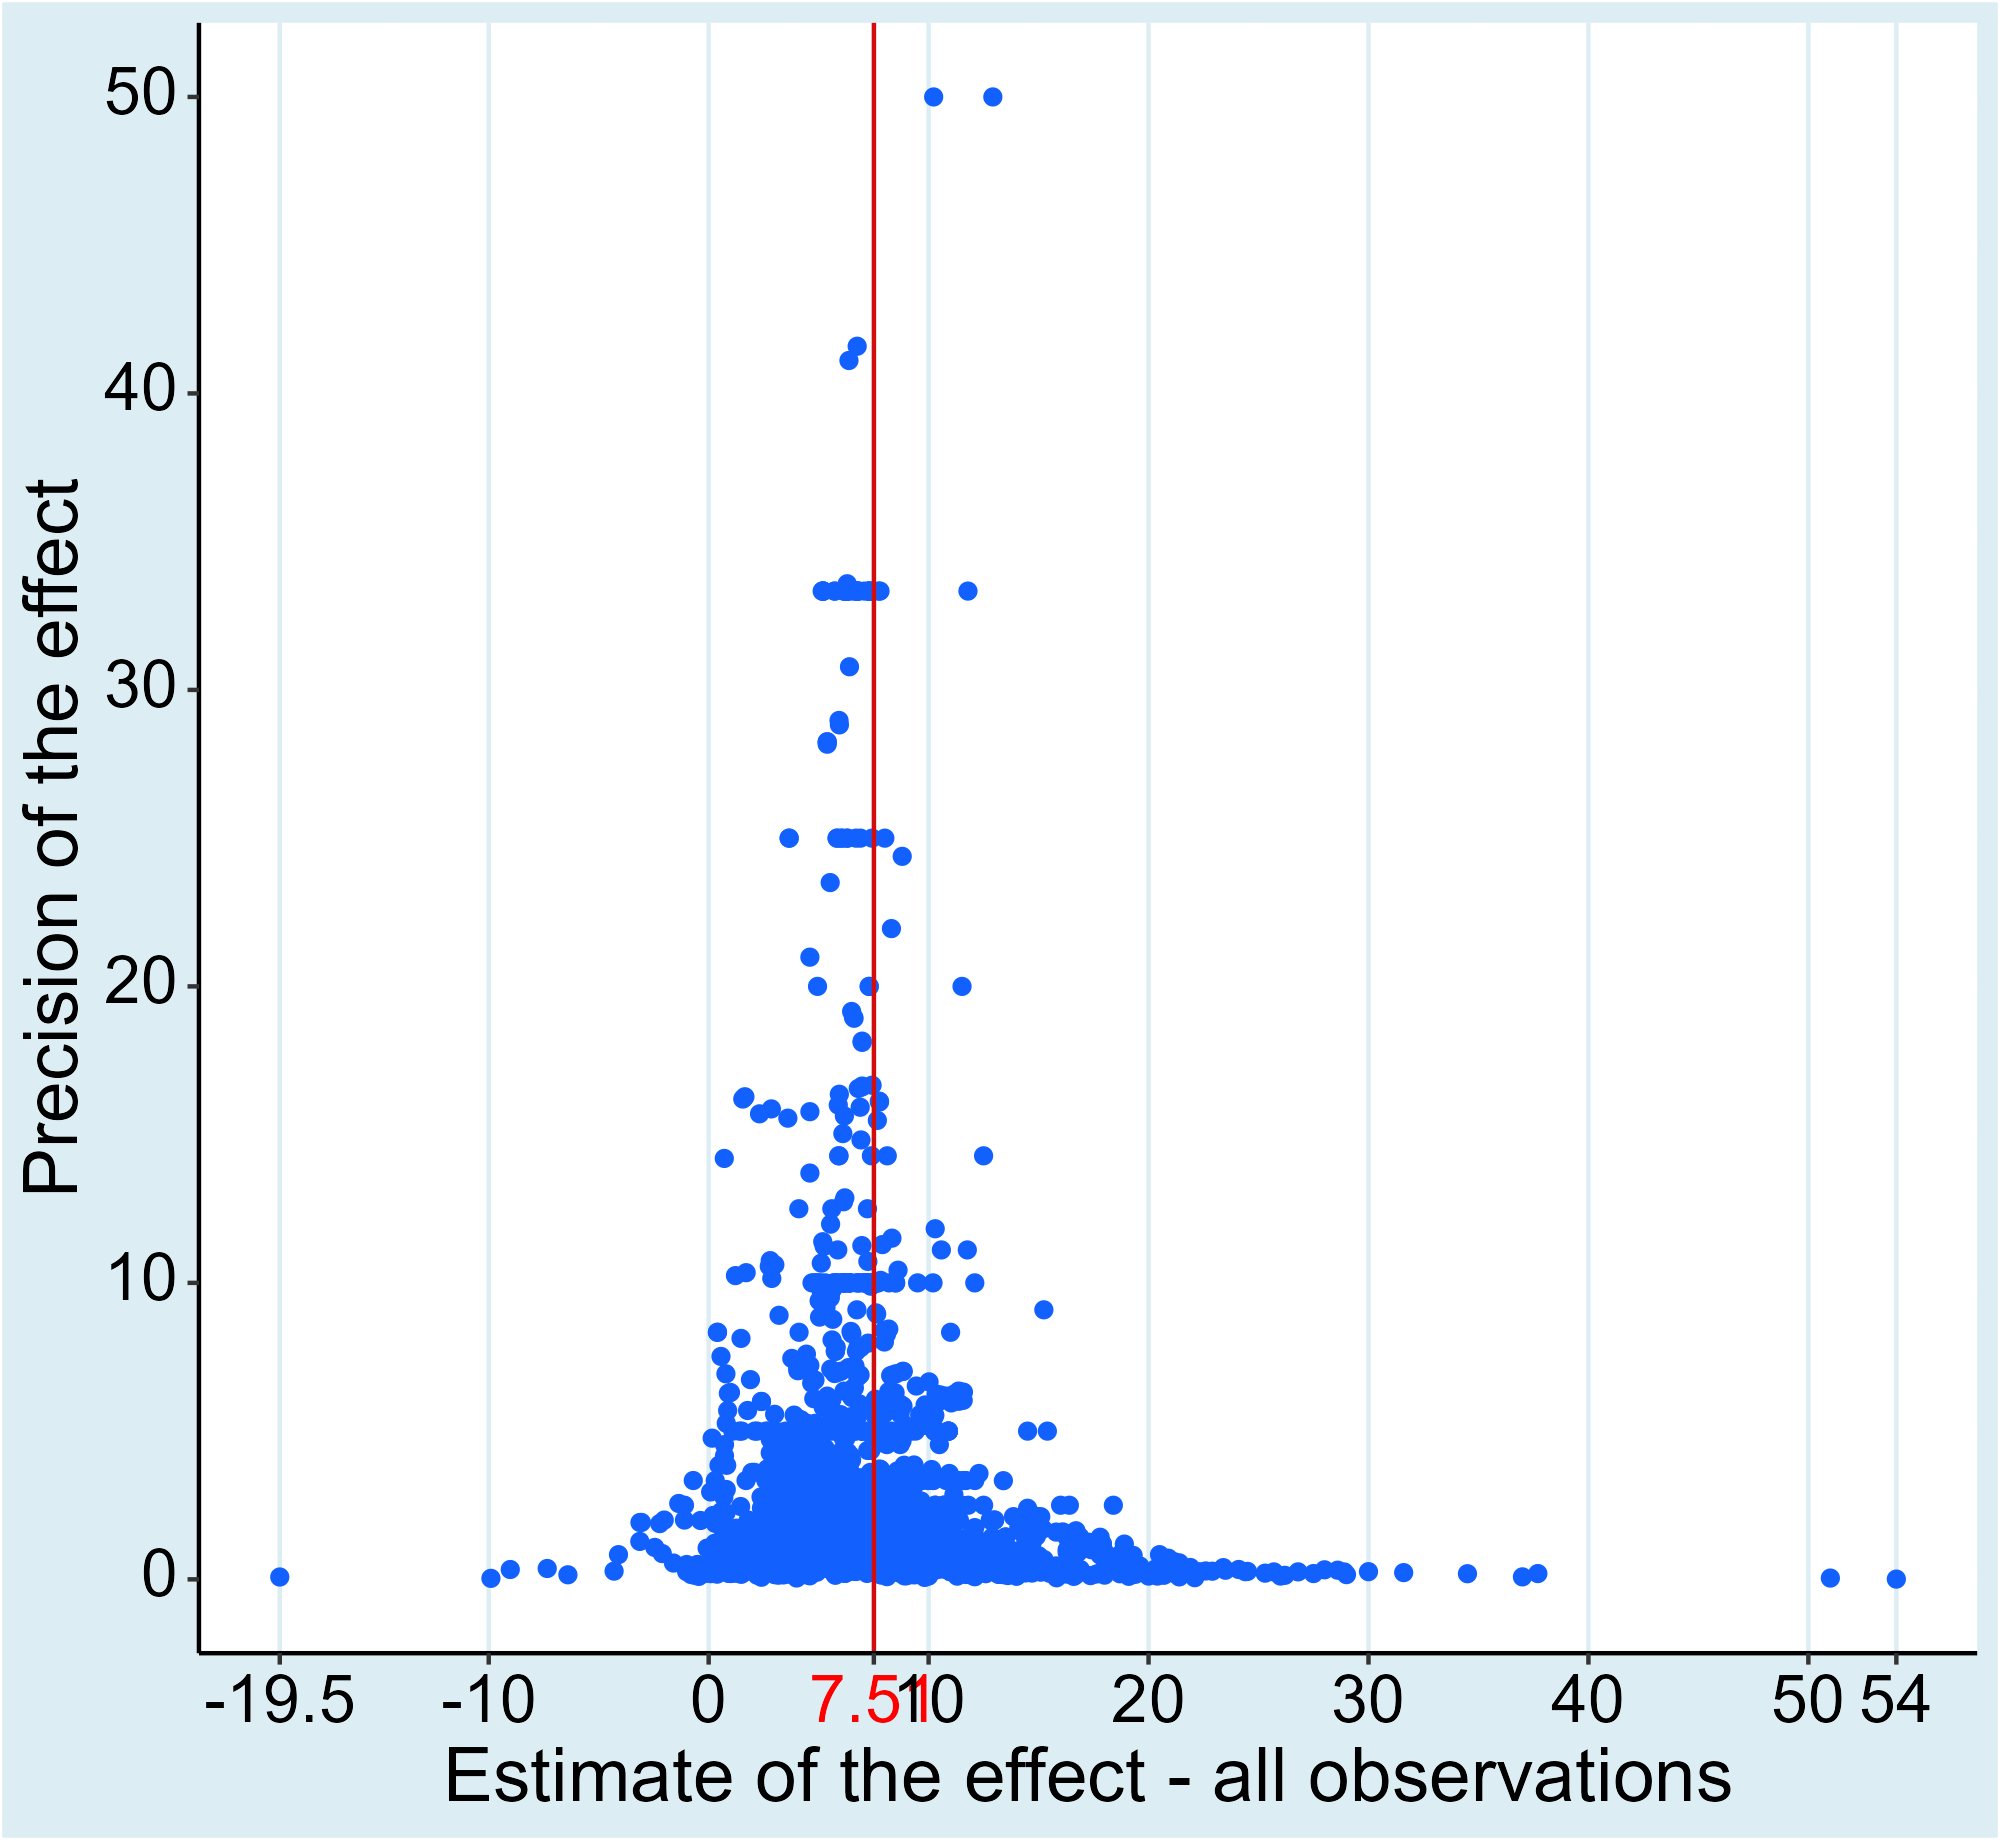
\includegraphics[width=0.95\linewidth]{Figures/funnel.png}
   \label{fig:funnel_plot_all} 
\end{subfigure}
\begin{subfigure}[b]{0.45\textwidth}
   \caption{Study medians}
   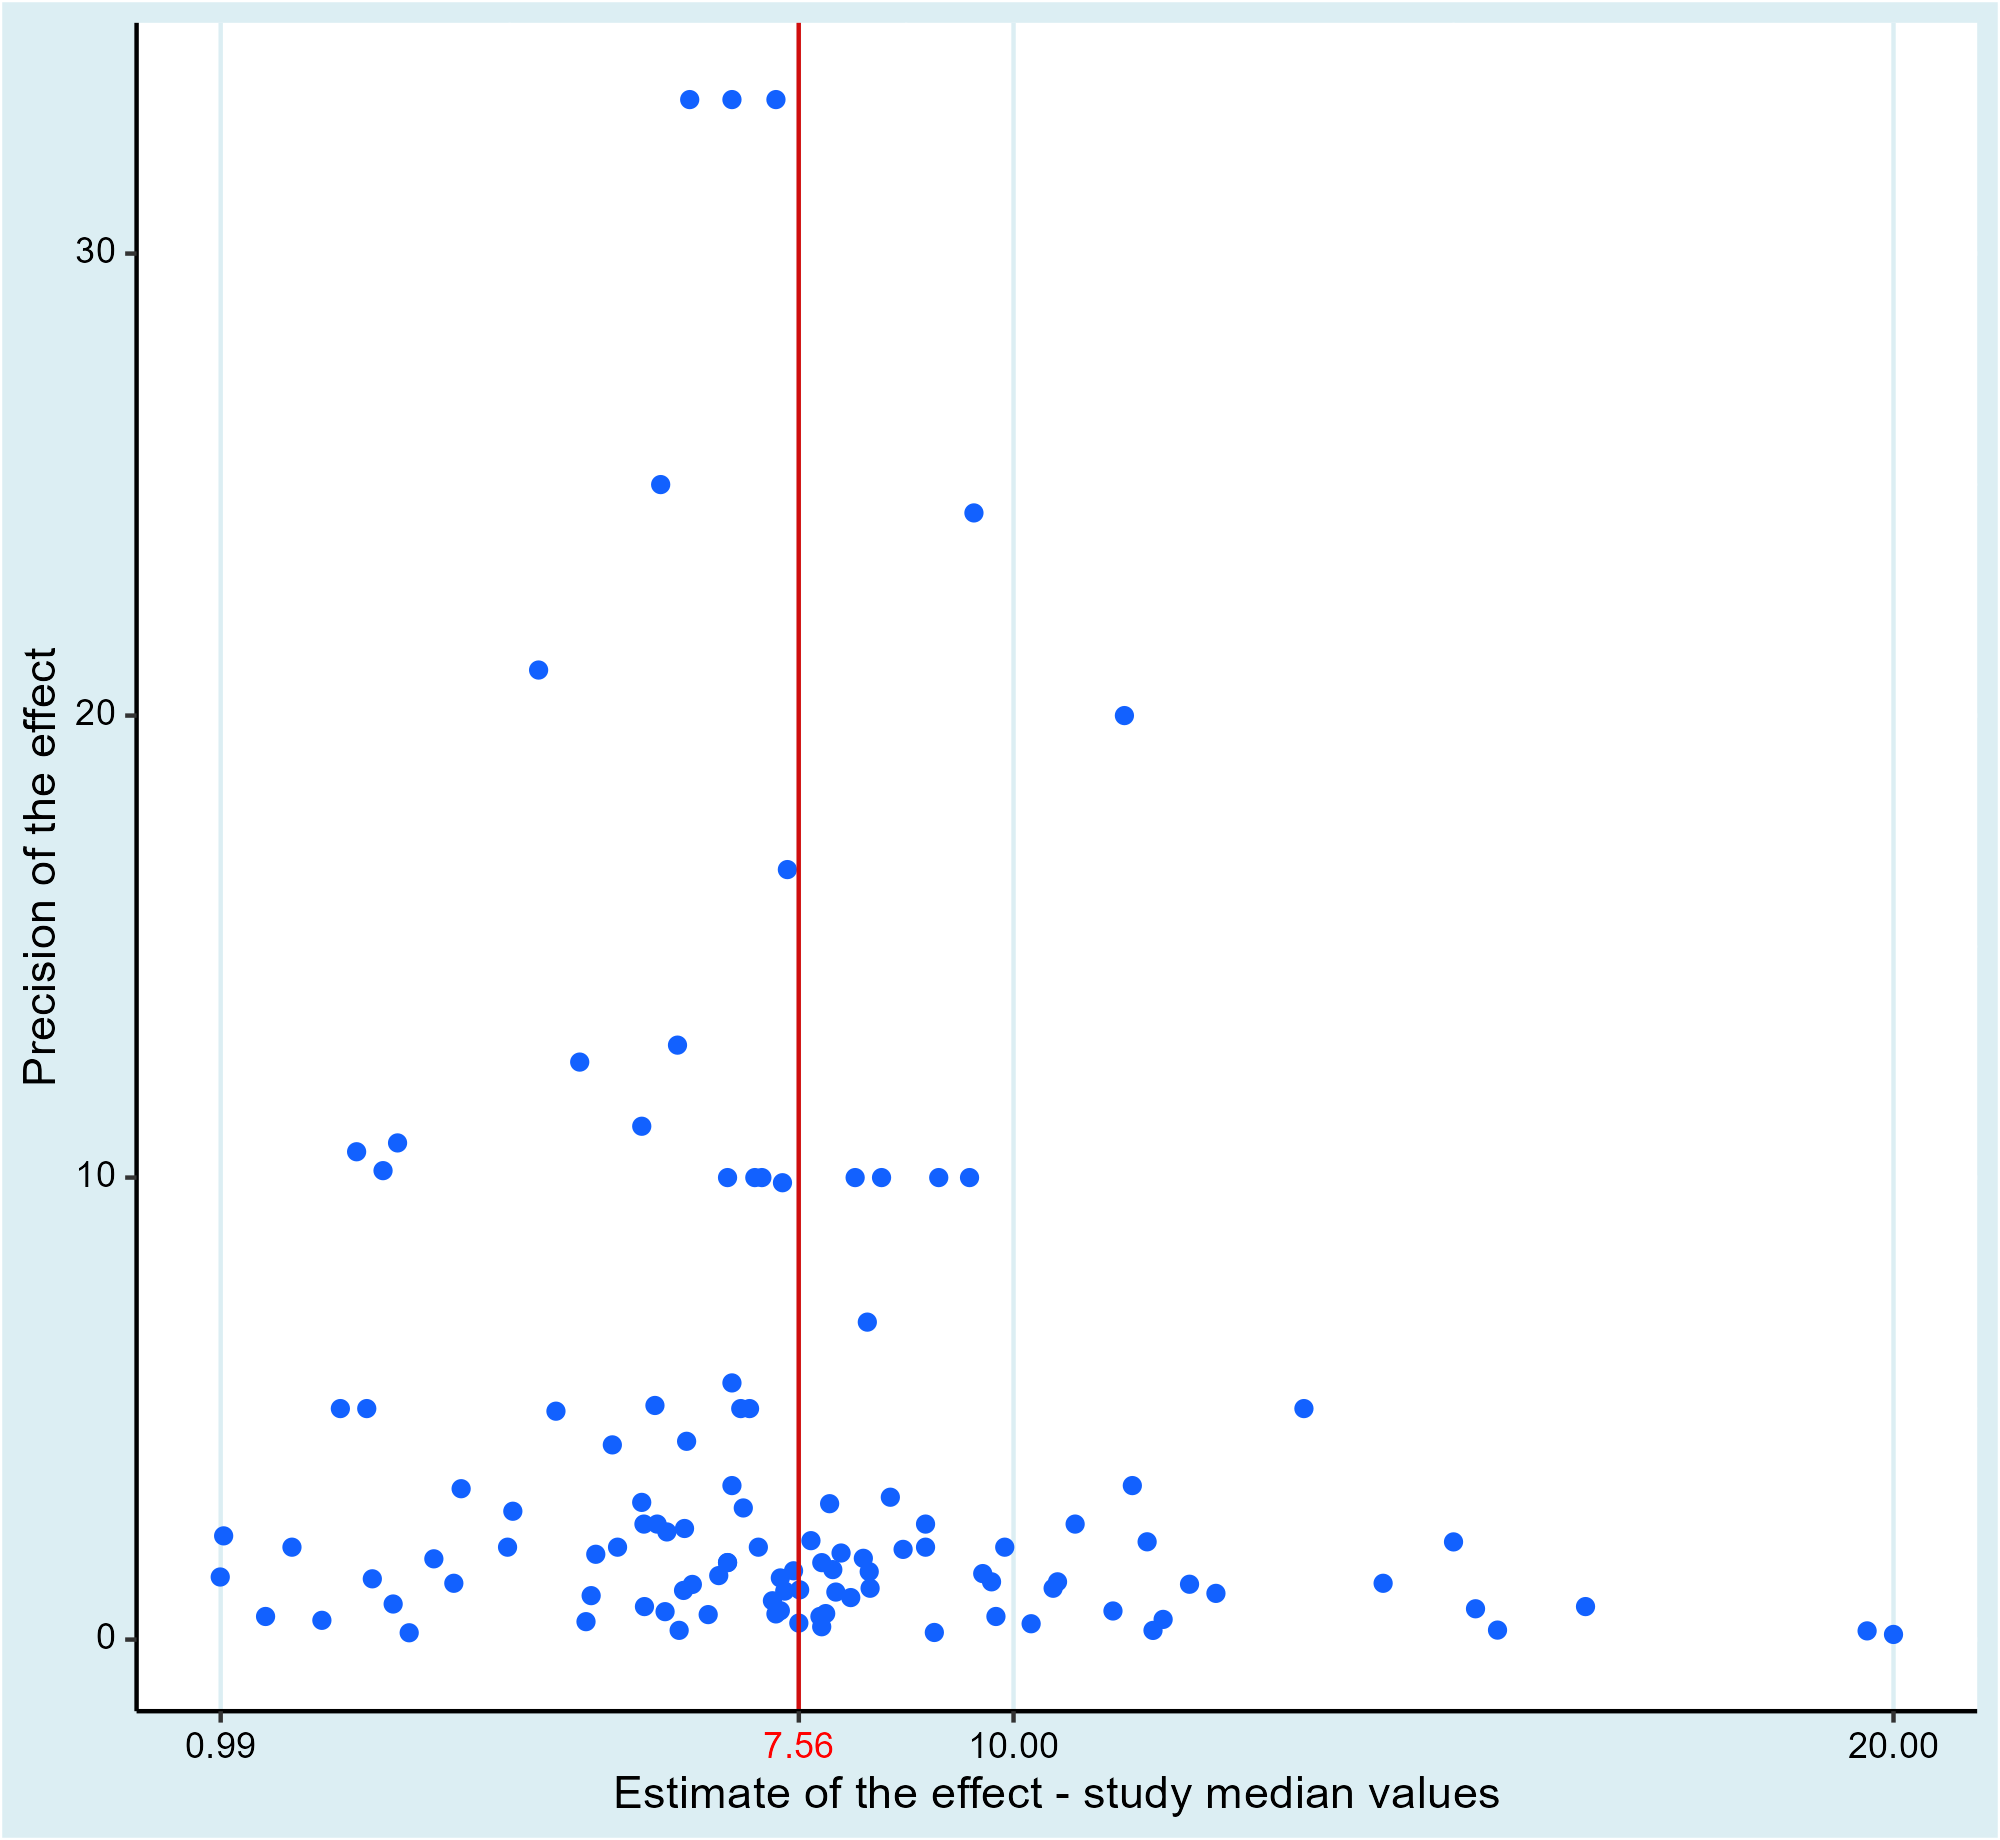
\includegraphics[width=0.95\linewidth]{Figures/funnel_medians.png}
   \label{fig:funnel_plot_medians}
\end{subfigure}
\end{center}\vspace{-0.6cm}
\captionsetup{width=0.85\textwidth, font = scriptsize}
\caption*{\emph{Note:} This figure displays two funnel plots as per \cite{Egger1997}, where the percentage returns to an additional year of schooling are plotted on the x-axis against precision on the y-axis, measured as $1/SE$ (Standard Error). Plot (a) shows the funnel plot for all observations within the data (1754 data points), while plot (b) shows only the medians of each study (115 data points). The red line marks the mean of these data points. In case of no publication bias, these funnel plots should be symmetrically centered around the true mean.}
\end{figure}

No apparent asymmetry nor holes appear at first glance in the plot with all observations. The less telling plot with study medians exhibits a little more "emptiness" at places, but we can take this simply as a cause of the lower observation count. The crucial takeaway from the latter plot is the lack of suspicious outliers in either direction. Despite this relative consistency, both graphs are perhaps a little more dispersed for higher precision values than the ideal shape might have it. In any case, this is far from enough evidence to claim the presence of publication bias and, contrarily, a hint that the data may be relatively normal.


\section{Funnel Asymmetry Tests}
\label{sec:linear_tests}

% Perhaps refer to the EK paper for theory on FAT-PET-PEESE tests

The funnel plot itself, albeit a quick and easy way of detecting obvious publication bias, is still a less precise method that relies on \textit{eye-balling} and subjective interpretation, both hardly rigorous ways of conducting research. To establish the results quantitatively and more robustly, I turn first to the \ac{FAT-PET} \citep{Egger1997, stanley2005beyond, stanley2008fatpet}.

These techniques test for the funnel plot asymmetry using a simple equation that regresses the effect on its standard error to uncover any correlation between the two. If such a correlation exists, it can be interpreted as a systematic relationship between the effect and its standard error, indicating publication bias. Algebraically, the relationship can be written as:

\begin{equation}\label{eq:fat_reg}
    S_{ij} = \beta_0 + \beta_1 * (SE_{S})_{ij} + u_{ij},
    \vspace{0.3cm}
\end{equation}

where $S$ represents the returns to schooling effect for the i-th observation of the j-th study in the dataset, and $SE_{S}$ corresponds to the effect's standard error. The slope coefficient, $\beta_1$, then measures the publication bias in the data, while the intercept coefficient, $\beta_0$, captures the "true" effect of returns to schooling corrected for publication bias. $u_{ij}$ stands for the error regression term. In the tables below, I will refer to the slope coefficient with the label \textit{Publication bias}, while the intercept will be labeled as \textit{Effect beyond bias}.

If no publication bias is present in the data, the slope coefficient will be either 0 or close to it. Conversely, higher absolute values would indicate the opposite correlation between the effect and its standard error, thereby suggesting publication bias is present in the data. This is motivated by the assumption that both the effect and its standard error should be, statistically speaking, drawn from an independent, statistically symmetrical distribution. However, practically speaking, this is rarely the case. 

The results of the funnel asymmetry tests can be viewed in \autoref{tab:PB-FAT}. Firstly, I include a simple \ac{OLS} model, followed by two models accounting for unobserved heterogeneity in the form of Fixed effect and Random effect estimators. Lastly, I introduce two models that weigh the equation, first by the inverse of the number of observations reported per study and second by precision. The motivation behind the last two models is to account for unobserved heterogeneity and heteroskedasticity, respectively. Four out of five of these methods find a statistically significant presence of publication bias, and all claim the underlying effect lies within the range of 6 and 7 percent, specifically between 6.294 and 6.708 percent. This indicates that the underlying effect might be slightly lower than the simple estimates' average, approximately by one percentage point. Furthermore, the lowest predicted value can be associated with the study-size weighted model (6.294), suggesting perhaps that studies of larger size drive the effect upwards. However, it is essential to note that this difference is relatively small compared to the other estimates. The discrepancy between the study-size weighted model and the fixed-effects model, the latter of which predicts the highest returns to education at 6.708 percent, is less than half a percentage point.

% Linear tests
\begin{table}[!t]
\centering
\footnotesize
\singlespace
\caption{Linear tests for publication bias}
\label{tab:PB-FAT}
\begin{tabular}{
@{\hskip\tabcolsep\extracolsep}
l*{5}{c}} %one left column, five center (*{} makes the cols inherit attributes)
\toprule
  \multicolumn{1}{l}{} &
  \multicolumn{1}{c}{\textbf{OLS}} & 
  \multicolumn{1}{c}{\textbf{FE}} &
  \multicolumn{1}{c}{\textbf{RE}} & 
  \multicolumn{1}{c}{\textbf{Study}} &
  \multicolumn{1}{c}{\textbf{Precision}} \\
\midrule

    Publication bias & 0.832*** & 0.746*** & 0.747*** & 1.169*** & 0.262 \\
    \emph{\hspace{0.2cm}(Standard error)} & (0.097)  & (0.060) & (0.058) & (0.121) & (0.425) \\
    \addlinespace[0.5em]
    Effect beyond bias & 6.408*** & 6.517*** & 6.708*** & 6.294*** & 6.540*** \\
    \emph{\hspace{0.2cm}(Constant)} & (0.118)  & (0.107) & (0.294) & (0.153) & (0.168) \\
    \addlinespace[0.5em]
    Observations & 1,754 & 1,754 & 1,754 & 1,754 & 1,754 \\
    
\bottomrule
\multicolumn{6}{>{\scriptsize}p{0.85\linewidth}}{\emph{Note:} The table displays the results obtained from estimating \autoref{eq:fat_reg} OLS = Ordinary Least Squares. FE = Fixed Effects. RE = Random Effects. Precision = Estimates are weighted by the inverse standard error. Study = Estimates are weighted by the inverse number of observations reported per study. Standard errors, clustered at the study level, are included in parentheses. ***p<0.01, **p<0.05, *p<0.1}
\end{tabular}
\end{table}


\section{Non-linear Tests}
\label{sec:nonlinear_tests}

The relationship between the effect and its standard error, as described in \autoref{eq:fat_reg}, is assumed to be linear in the funnel asymmetry tests. However, it is crucial to acknowledge that this assumption does not always hold. In cases where the relationship behaves less straightforwardly, the \ac{FAT-PET} tend to underestimate the underlying effect if it differs from zero \citep{stanley2014meta}. In the context of my data, this concern may be valid since most of the data points are positive and occasionally even reach double digits. To address potential non-linear forms of the relationship that may appear in the data, I present six techniques that relax the linearity assumption. 

The first is the \ac{WAAP}, introduced by \cite{Ioannidis2017Waap}. Their proposition involves the application of unrestricted \ac{WLS} only on observations of adequately powered studies. "Power" here refers to a study's ability to detect whether an effect if it is truly present in the data. The more power a study has, the bigger its reliability. In technical terms, the power is calculated using the statistical significance of estimates and then compared to their standard errors. As per the original paper, I kept only the estimates of studies that display power over 80\%. Strikingly, 1469 out of the 1754 estimates in my dataset get identified as adequately powered. Using these estimates, \ac{WAAP} then proposes an estimate of 6.9\% which is slightly higher than any of the linear models presented in \autoref{tab:PB-FAT}.

The second approach, proposed by \cite{Stanley2010Top}, entails discarding 90\% of data and keeping only the top 10 percent with the highest precision. This somewhat paradoxical approach stems from the idea that most researchers use statistical significance as the primary benchmark for deciding whether to publish the estimate. \cite{Stanley2010Top} show that if most of the less precise estimates are discarded, the publication bias within the data sample drops considerably. In my data, 10\% of estimates correspond to 176 observations. The Top10 model yields a modest result of 6.439\%.

\cite{Furukawa2019Stem} chooses a similar tactic by selecting a specific number of the most precise estimates. The cutoff is determined by minimizing mean square error; this aims at striking a balance between variance/efficiency and bias. The selected points from what is referred to as "stem" are those with the lowest mean square error. You may find a visual representation of this method in \autoref{fig:stem}. The coefficient of returns to education suggested by this approach is 7.2\%, the highest among all the proposed regression-based results thus far.

\sidecaptionvpos{figure}{t}
\begin{SCfigure}
\centering
\captionsetup{font = scriptsize}
\caption[Stem-based method]{\vspace{0.5cm}Stem-based method\\ \emph{Note:} This figure displays a non-linear estimation of the true effect \citep{Furukawa2019Stem}. The main effect, labeled \textit{Coefficient $\beta$}, is plotted on the x-axis against precision, calculated as $log(SE)$ (Standard Error). The yellow diamond and the whiskers of the same color denote the 95\% confidence interval of the stem-based estimate of the effect. The dark grey line indicates the predicted estimates throughout various levels of data, while the purple diamond shows the minimal precision value above which lies the stem. The blue circles then represent the individual effect estimates.}
\label{fig:stem}
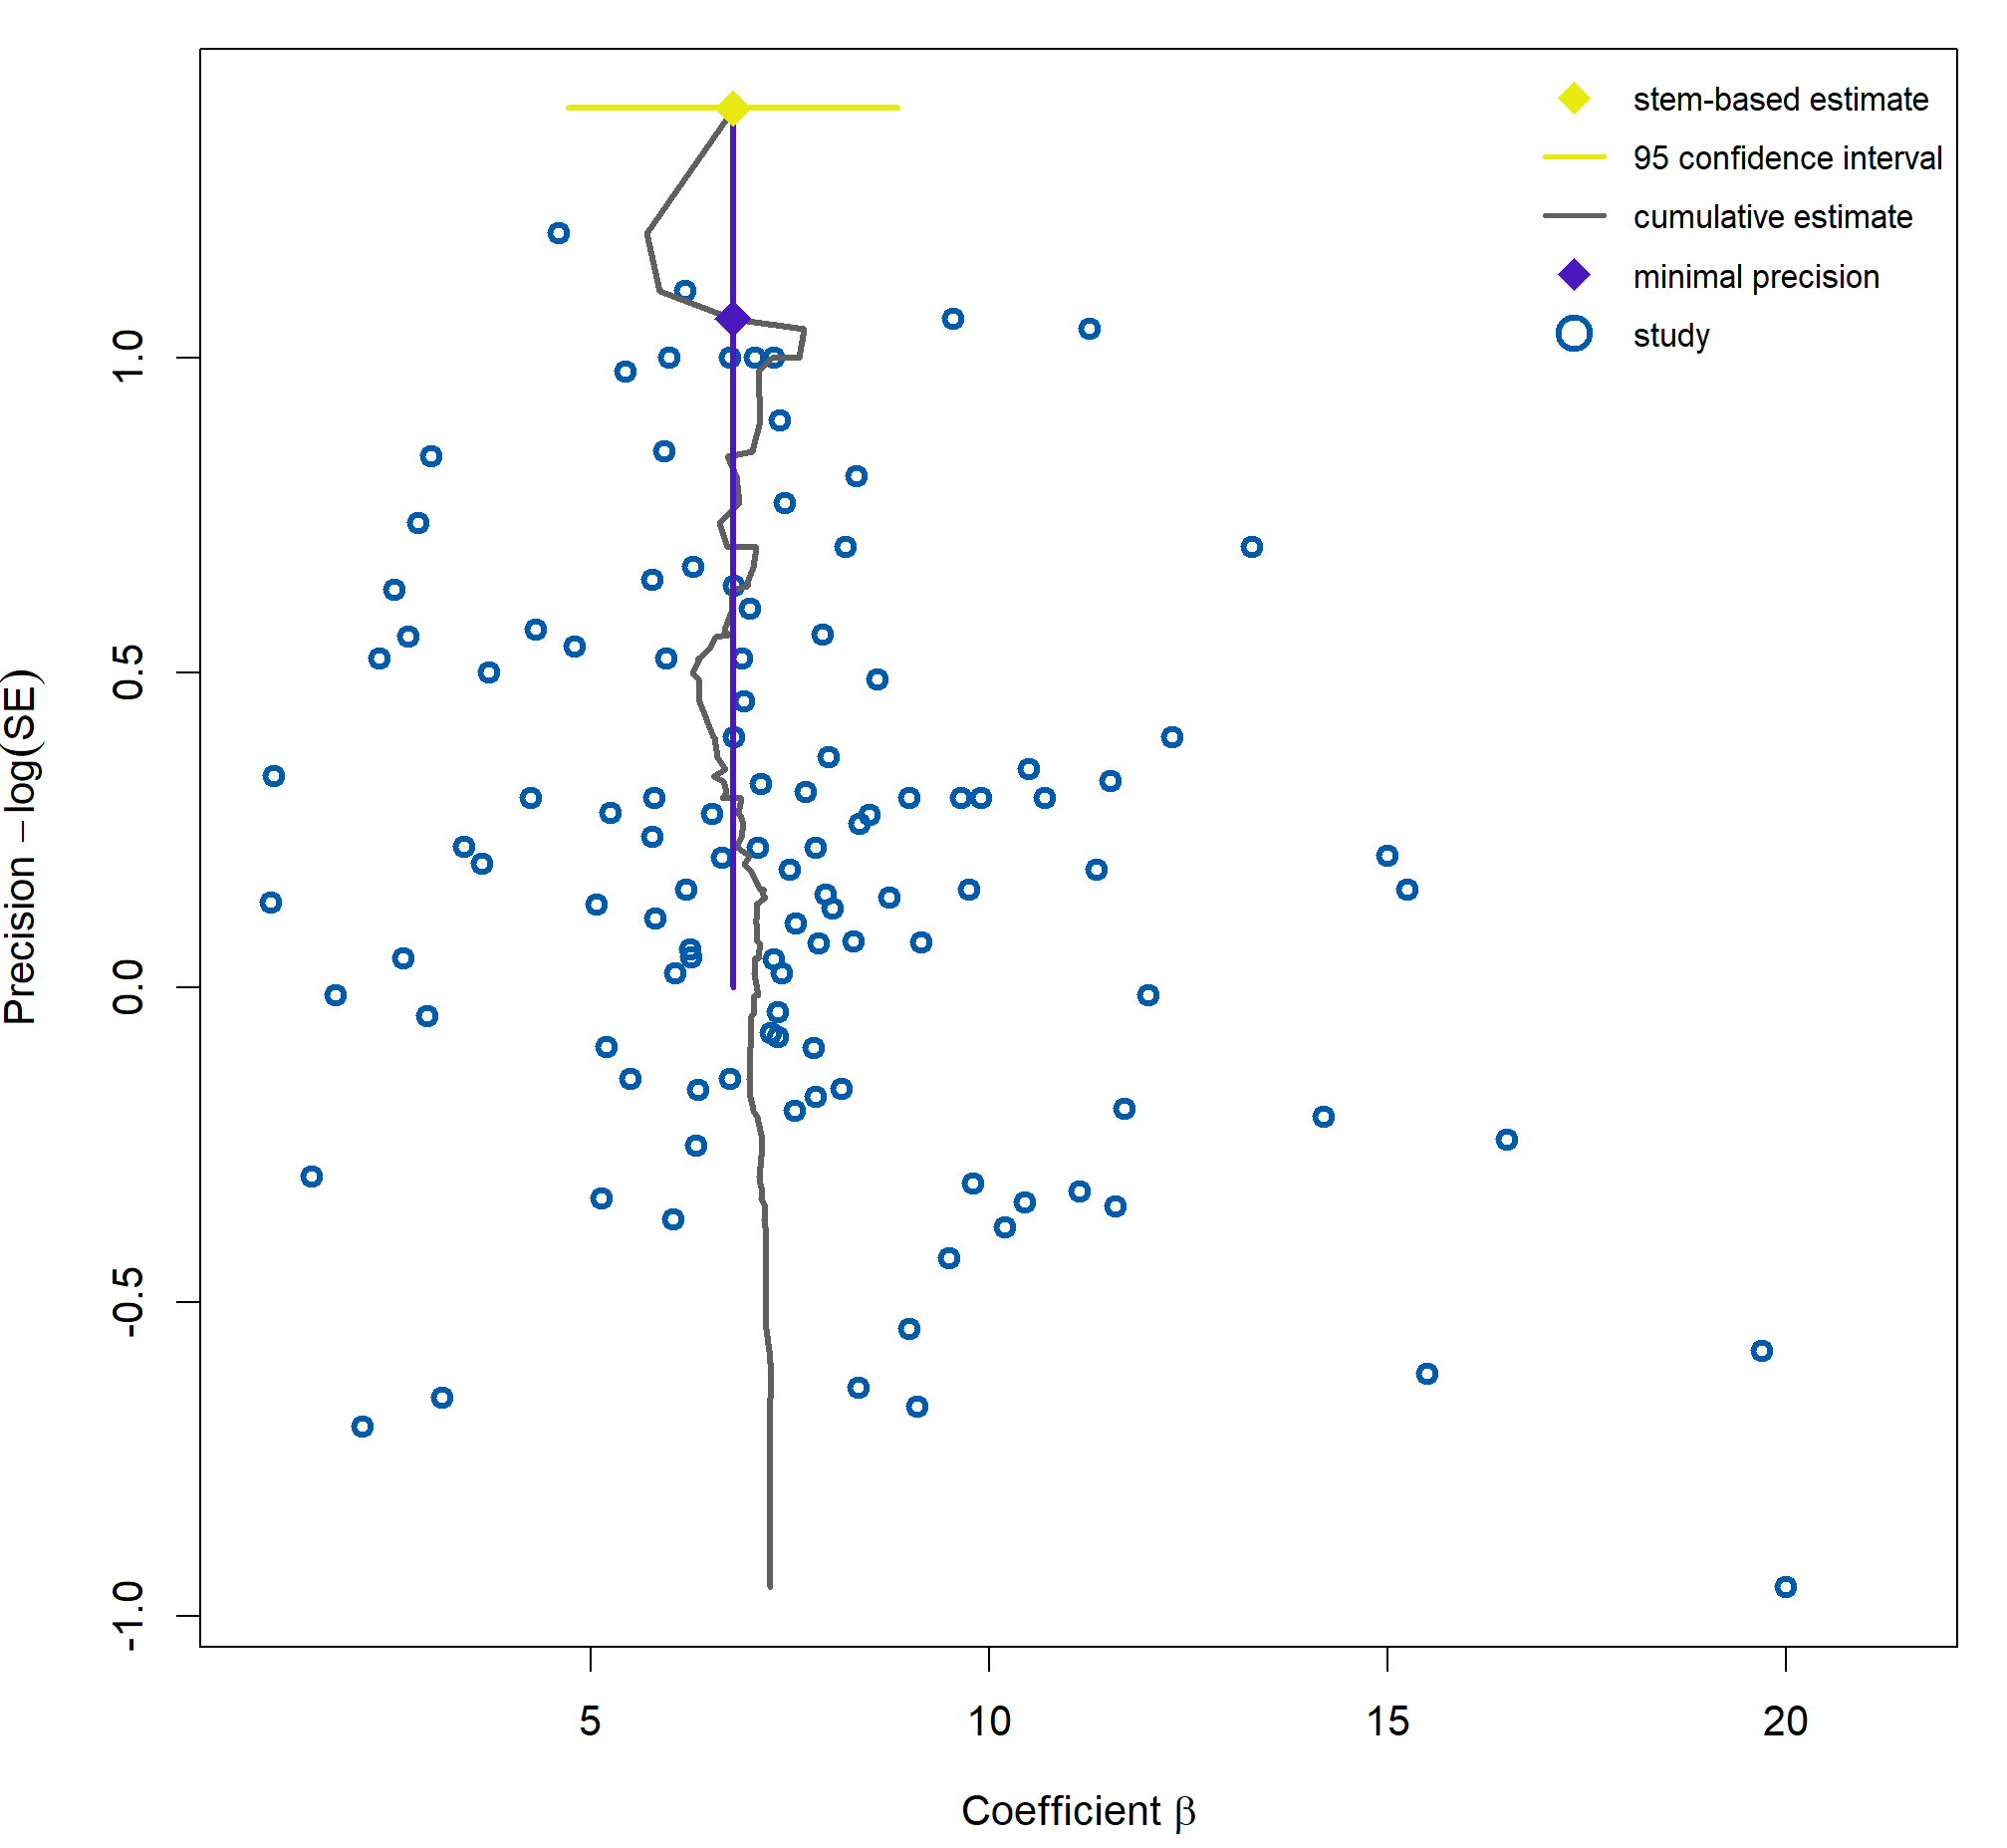
\includegraphics[width=0.5\textwidth]{Figures/stem.png}
\end{SCfigure}

Further, I estimate the Hierarchical Bayes model by \cite{Allenby2006Hier}. The procedure employs Bayesian statistics to leverage variability within individual studies to determine the weights of individual observations aggregated at the study level. The model parameters get treated as random variables instead of fixed numbers, allowing for variability at multiple levels within the dataset. As such, different units can have comparable sharing strength, allowing for more robust estimates. The hierarchical part stems from the fact that priors are specified using another model (called hyperprior) instead of a direct specification, as is usually done in Bayesian modeling. This complex multi-level modeling framework yields an estimate of 6.8\% in my case. Additionally, the analysis suggests the presence of publication bias at a significance level of 1\%.

% Non-linear tests
\begin{table}[!b]
\centering
\footnotesize
\singlespace
\caption{Nonlinear tests for publication bias}
\label{tab:N-L}
\begin{tabular}{
@{\hskip\tabcolsep\extracolsep}
l
*{6}{c}
@{}
} %0.15 0.65
\toprule
  \addlinespace[0.5em]
  \multicolumn{1}{c}{} &
  \multicolumn{1}{c}{\textbf{WAAP}} & 
  \multicolumn{1}{c}{\textbf{Top10}} &
  \multicolumn{1}{c}{\textbf{Stem}} & 
  \multicolumn{1}{c}{\textbf{Hier}} &
  \multicolumn{1}{c}{\textbf{AK}} &
  \multicolumn{1}{c}{\textbf{Kink}} \\
\midrule
    Publication bias & & & & 0.503*** & P = 2.764 & 0.262 \\
    & & & & (0.168) & (0.107) & (0.39)\\
    \addlinespace[0.5em]
    Effect beyond bias & 6.9*** & 6.439*** & 7.2*** & 6.801*** & 6.548*** & 6.54*** \\
    & (0.092) & (0.548) & (1.186) & (0.266) & (0.091) & (0.054) \\
    \addlinespace[0.5em]
    Observations & 1,754 & 1,754 & 1,754 & 1,754 & 1,754 & 1,754 \\
\bottomrule
\multicolumn{7}{>{\scriptsize}p{0.95\linewidth}}{\emph{Note:}  The table reports estimates of the effect beyond bias using six non-linear methods and estimates of the publication bias obtained using two of these methods. WAAP = Weighted Average of the Adequately Powered \citep{Ioannidis2017Waap}. Top10 = Top10 method by \cite{Stanley2010Top}. Stem = the stem-based method by \cite{Furukawa2019Stem} where P represents the probability of results insignificant at 5\% being published relative to the probability of the significant ones at the same level. Hier = Hierarchical Bayes model \citep{Allenby2006Hier}. AK = \cite{Andrews2019Selection}'s Selection model. Kink = Endogenous kink model by \cite{Bom2019Kink}. Standard errors, clustered at the study level, are included in parentheses. ***p<0.01, **p<0.05, *p<0.1 }
\end{tabular}
\end{table}


The next test is the Selection model proposed by \cite{Andrews2019Selection}. The authors argue that the publication probability for estimates remains constant at similar levels of statistical significance, a concept called "conditional publication probability." Once a certain statistical significance threshold is crossed, the publication probability changes. \cite{Andrews2019Selection} then demonstrate how this probability can be calculated non-parametrically, and utilizing the inverse of this probability as new weights, they obtain a non-biased distribution of the estimates. Using a t-distribution at the 5\% significance level (cutoffs for $p(.)$ set to 1.96), I obtain the result of 6.548\%. The method also proposes that estimates at the 5\% significance level are more likely to be published than insignificant ones (P = 2.764).

As the last of the non-linear techniques testing for publication bias, I add the \ac{EK} model introduced by \cite{Bom2019Kink}. Using the argument that the publication bias is usually absent for sufficiently large studies, the \ac{EK} model finds a cutoff value below which publication bias should not appear. \cite{Bom2019Kink} then fit a piecewise linear regression with a kink at this cutoff point, allowing non-linearity in the model. An advantage of this approach is that this method reduces to a simple linear model as the effect approaches zero, where said linear methods perform well. As such, the \ac{EK} approach should provide more robust results than its linear counterpart. In my case, the suggested value of the main effect is 6.54\%, which falls right into the average of the rest of the (both linear and non-linear) results. The model also provides a non-significant estimate of the presence of publication bias. This marks the last of non-linear methods; all of the results obtained from these estimations can be found in \autoref{tab:N-L}.

All but one of the six models propose a statistically significant effect beyond bias within the 6 to 7 percent range. Only the stem-based method suggests a coefficient for returns to education above 7\% (specifically, 7.2\%). These results align with the linear approach and confirm the behavior observed thus far. The Hierarchical Bayes indicates a strong presence of publication bias, while the Endogenous Kink method result is insignificant. Finally, the Selection model proposes that results at the 5\% significance level have a considerably higher chance of publication than insignificant ones.


\section{Tests Without the Exogeneity Assumption}
\label{sec:exo_tests}

Until now, the publication bias tests have been based on the assumption that the correlation between the effect and the standard error indicates publication bias. However, this introduces, by definition, endogeneity into the equation. To see how this issue can be treated, it is essential to understand how it arises in the first place.

The correlation in the data, and thus endogeneity, can come from several sources. First, it could be a simple measurement error or wrong calculation procedure that introduces correlation into the data; the standard error, too, is an estimate, after all. Second - this is what the publication bias gets associated with perhaps the most - the endogeneity may arise from a conscious and deliberate tampering of the standard error to improve significance. And lastly, any unobserved heterogeneity may also introduce correlation, this time in the form of inherent methodological differences that may systematically influence the results. To display the estimate-error relationship clean of endogeneity, I utilize two techniques - \ac{IV} regression and p-uniform* \citep{vanAert2021puni}.

First, the \ac{IV} regression, for which we need an instrument. The criteria for finding a valid one are relatively simple - it should be a metric that somehow captures the behavior of (correlates with) standard error while having no relationship to the estimate. Using such metric, it should be possible to derive the publication bias coefficient ($\beta_1$ from \autoref{eq:fat_reg}) not poisoned by endogeneity. Several instruments appear valid here, including $\frac{1}{\sqrt{n_{\text{obs}}}}$, $\frac{1}{n_{\text{obs}}}$, $\frac{1}{n_{\text{obs}}^2}$, and $\log(n_{\text{obs}})$, where $n_{\text{obs}}$ stands for the number of observations associated with each estimate. The number of observations variable holds several inherent properties that make all these instruments valid options. Firstly, the size of an experiment, or the number of subjects in the study, does not directly change the population-wide effect. If such a true effect exists, it should be independent of how many subjects we include in the analysis. Secondly, the standard error decreases as the sample size increases. This is a fundamental principle of statistics. In other words, the more subjects there are in the study, the bigger the confidence that the findings based on that sample are close to the results had the whole population been used for calculation.

Still, which of these four proposed instruments is the best? To find out, I wrote a helper function in R that automatically detects the best-performing instruments based on the results of several specification tests. These are, namely, the Underidentification test, the Weak identification test, the Stock-Yogo weak ID test, and the Sargan statistic.\footnote{All of these specification tests are in-built into the \textit{ivreg} function of the {ivreg} R package, which I used to estimate this method. Source \href{https://cran.r-project.org/package=ivreg}{here}.} I omit the numeric results of these tests as they are not crucial for interpreting the results, and only mention that $\frac{1}{\sqrt{n_{\text{obs}}}}$ performed the best out of the four instruments. Using this instrument, the \ac{IV} regression gives 6.155\% as an estimate of returns to education, which coincides with the estimates computed up to this point.

%Table with the results of the IV/p-uni* tests
\begin{singlespace}
\begin{footnotesize}
\begin{longtable}[!htbp]{
@{\hskip\tabcolsep\extracolsep}
l
*{2}{c}
@{}
}
\caption{Relaxing the exogeneity assumption}  \label{tab:IV-p}\\
\toprule
  \multicolumn{1}{l}{} &
  \multicolumn{1}{c}{\centering{\textbf{IV}}} &
  \multicolumn{1}{c}{\centering{\textbf{p-uniform*}}} \\
\midrule
\endfirsthead
    Publication bias    & 1.295*** & L = 9.439\\
     & (0.281) & (p = 0.002)\\
    \addlinespace[0.5em]
    Effect beyond bias  & 5.813*** & 9.520***\\
     & (0.354)  & (3.291)\\
    \addlinespace[0.5em]
    Observations & 1,754 & 1,754 \\
    
\bottomrule
\multicolumn{3}{>{\scriptsize}p{0.5\linewidth}}{\emph{Note:} IV = Instrumental Variable Regression; one over the square root of the number of studies is used as an instrument for the standard error. Standard errors, reported in parentheses, are also clustered at the study level. p-uniform* = method proposed by \cite{vanAert2021puni}; L represents the publication bias test t-statistic; the corresponding p-value can be found in parentheses. ***p<0.01, **p<0.05, *p<0.1}
\end{longtable}
\end{footnotesize}
\end{singlespace}

As another way of estimating the effect-error relationship without prior assumptions about its form, I turn to the p-uniform* method. This approach, proposed by \cite{vanAert2021puni}, builds on the p-uniform method \citep{van2016conducting}. The core idea stems from the principle that the p-values in the data should be uniformly distributed at the true effect size. This line of thinking requires no assumptions about the form nor correlation of the relationship and helps search for publication bias in a novel way. The p-uniform* method, then, improves the p-uniform approach in efficiency, precision, and between-study variance detection. In my data, this technique estimates the effect to be 9.52\% and indicates the presence of publication bias, both at high levels of significance. Results of both methods can be found in table \autoref{tab:IV-p}. 

While the instrumental variable approach proposes rather sensible results, the p-uniform* is an outlier among previous estimates. This is perhaps more perplexing given that, were between-study to cause the effect's overinflation, p-uniform* is a method that should account for this. Among various possibilities, these results may stem from a calculation error or, perchance, a hidden trend or anomaly within the data, which is hard to detect. Suffice it to say I dug into the calculation multiple times to validate that all specifications and other inputs were sensible; still, I could not find anything out of the ordinary. As such, I present the results with a grain of salt but believe them to be fully valid.


\section{Caliper Tests}
\label{sec:caliper}

Yet another method I will use to search for deviations from normality in the reported literature results are Caliper tests, developed by \cite{gerber2008caliper}. Their proposed approach does not assume any prior relationship between the effect and the standard effect, similar to the tests from \autoref{sec:exo_tests}. Here, t-statistics are subjected to scrutiny, and the authors argue that upon looking at the immediate vicinity of a conventional significance level, no structural breaks in the distribution of t-statistic should occur. In other words, the t-statistic distribution should, in theory, behave relatively normally, and any large jumps may indicate the presence of publication bias.

Going into more detail, \cite{gerber2008caliper} suggest observing the number of t-statistics around significant t-statistic thresholds, such as 1.69 or 1.96, in intervals of varying widths, called Caliper widths. If, within any half of that interval, there is a significant imbalance in the number of t-statistics compared to the other half, it indicates a structural break around the observed threshold. In my case, I will explore how the t-statistics included from all studies of the data set behave around thresholds 1.645, 1.96, and 2.58, with Caliper widths of 0.05, 0.1, and 0.2. The choice of the latter is arbitrary, while the choice of the former stems from the fact that the three values correspond to the 1\%, 5\%, and 10\% significance levels. In academia, it is a common practice to append asterisks to results when presenting estimates together with their standard errors and hence, t-statistics. Unfortunately, this practice inadvertently emphasizes results marked with these asterisks \citep{simmons2011false}. As such, researchers may be tempted to include these asterisks in their tables at the cost of honesty, leading them to tamper with their figures (most notably standard errors). Consequently, publication bias may arise.

In \autoref{fig:t_hist}, you may find the distribution of t-statistics in my data, while \autoref{tab:caliperA} reports the results of Caliper tests described in the previous paragraphs.


%T-statistic distribution

\begin{figure}[!b]
\centering
\caption{The distribution of t-statistics is heavily skewed}
\label{fig:t_hist}
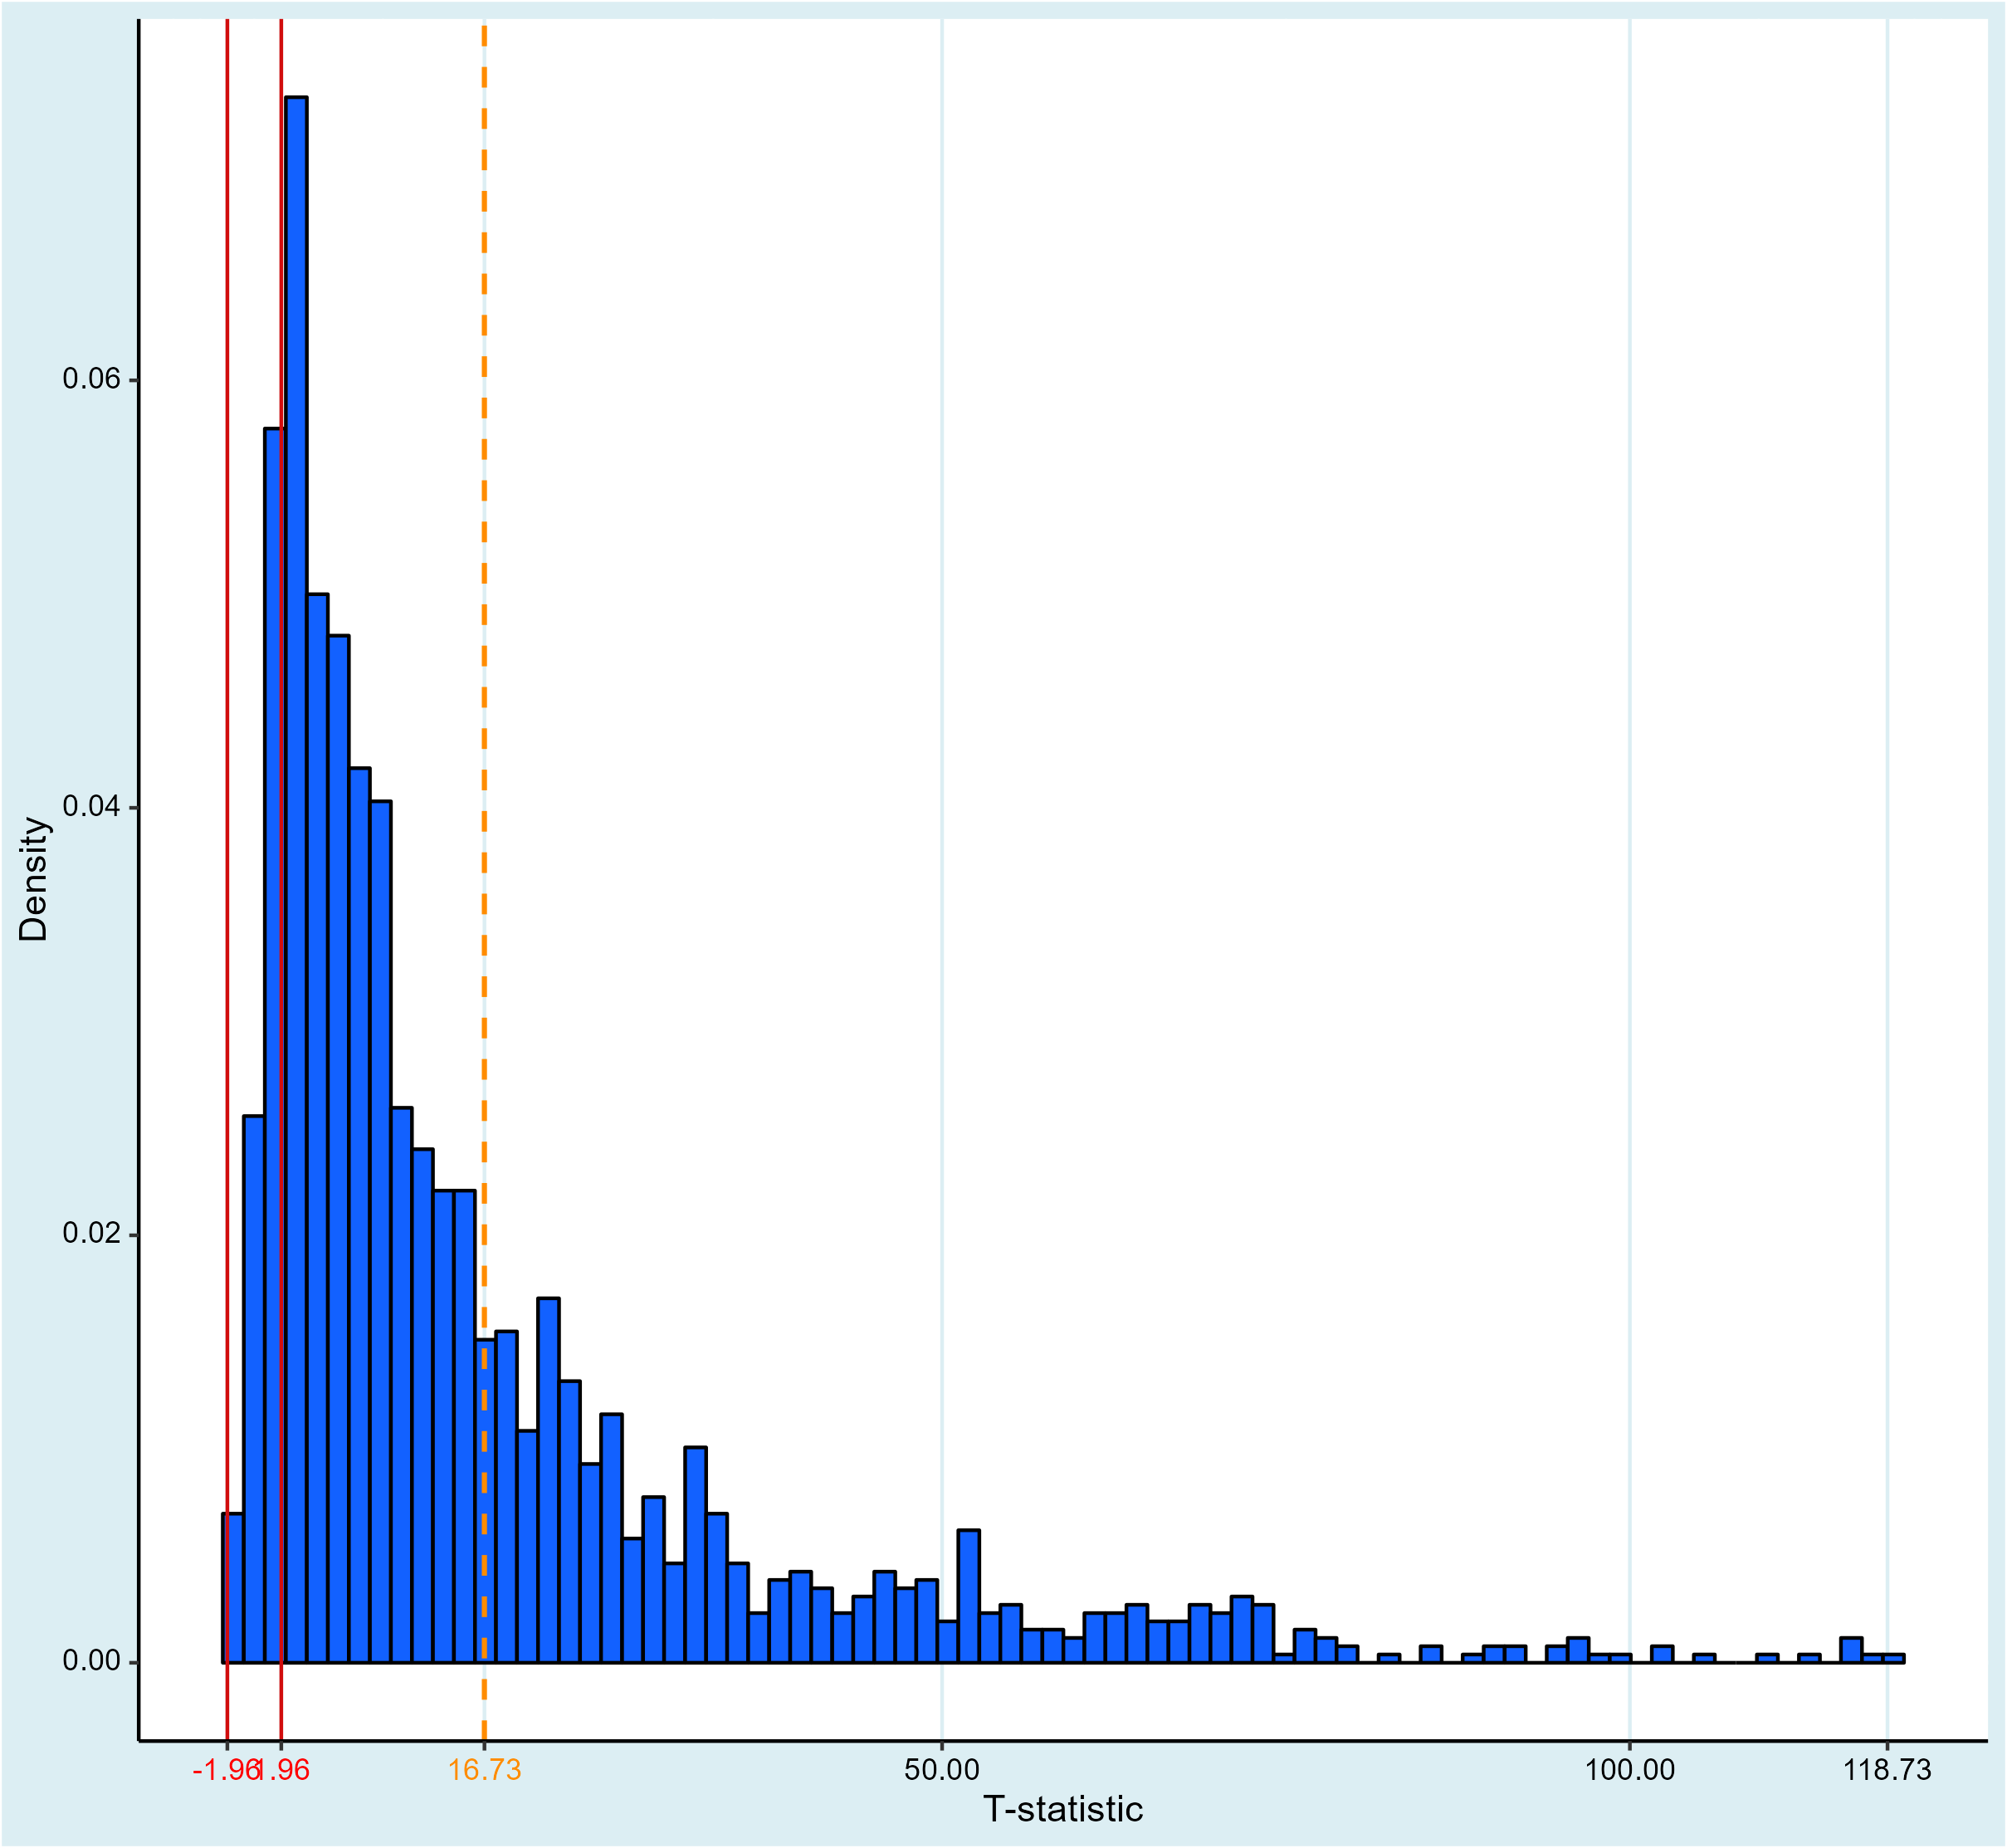
\includegraphics[width=0.7\textwidth]{Figures/t_hist.png}
\captionsetup{width=0.7\textwidth, font = scriptsize}
\caption*{\emph{Note:} The figure depicts the distribution of t-statistics associated with estimates within the dataset. The two red lines mark the critical significance values -1.96 and 1.96 (from left to right) at the 95\% confidence level. The dotted orange line represents the mean t-statistic within the data. Outliers are hidden for clarity of presentation, but we included them in the calculations.}
\end{figure}


% Results of Caliper tests
\afterpage{
\begin{singlespace}
\begin{footnotesize}
\begin{longtable}[!htbp]{
@{\hskip\tabcolsep\extracolsep}
l
*{3}{c}
@{}
}
\caption{Caliper tests at values 1.645, 1.96 and 2.58}  \label{tab:caliperA}\\
\toprule
  \multicolumn{1}{l}{} &
  \multicolumn{1}{c}{\centering{\textbf{Threshold 1.645}}} &
  \multicolumn{1}{c}{\centering{\textbf{Threshold 1.96}}} &
  \multicolumn{1}{c}{\centering{\textbf{Threshold 2.58}}} \\
\midrule
\endfirsthead
 Caliper width 0.05 & 0.517 & 0.243 & 0.152 \\
 & (0.084) & (0.063) & (0.046) \\
 \hspace{0.2cm}$n_{1}/n_{2}$ & 6 / 1 & 8 / 9 & 7 / 11 \\
 \addlinespace[0.5em]
 Caliper width 0.1 & 0.467 & 0.23 & 0.183 \\
 & (0.069) & (0.051) & (0.037) \\
 \hspace{0.2cm}$n_{1}/n_{2}$ & 10 / 3 & 11 / 14 & 13 / 15 \\
 \addlinespace[0.5em]
 Caliper width 0.2 & 0.455 & 0.241 & 0.162 \\
 & (0.036) & (0.033) & (0.025) \\
 \hspace{0.2cm}$n_{1}/n_{2}$ & 30 / 10 & 24 / 30 & 23 / 35 \\
\bottomrule
\multicolumn{4}{>{\scriptsize}p{0.9\linewidth}}{\emph{Note:} The table shows the results of three sets of Caliper tests by \cite{gerber2008caliper} These sets are carried out around t-statistic thresholds of 1.645, 1.96 and 2.58, which correspond to the 1\%, 5\%, and 10\% t-statistic significance levels. Caliper width denotes the width of the interval around the t-statistic, e.g., Caliper width 0.05 for threshold 1.96 means $t\in<1.91;2.01>$. A test statistic of 0.243 means that roughly 74\% of estimates appear above the threshold and roughly 26\% below it. $n_1/n_2$  = number of observations above/below the threshold. Standard errors, clustered at the study level, are included in parentheses.}
\end{longtable}
\end{footnotesize}
\end{singlespace}
}

Two quick notes about the results are in order. First, there are very few (only 34 out of the 1754 observations) estimates with negative t-statistics. Looking at the distribution from a purely statistical standpoint, it appears peculiar that the other 1730 are all associated with a positive t-statistic. From a practical perspective, however, this makes a lot of sense if we presume that the true effect indeed lies around 7\%. This assumption appears quite feasible, given the consistency of the tests carried out in the previous sections.

The second note should be addressed to the results of the Caliper tests. The jumps around thresholds could be described as \textit{striking}, \textit{considerable}, and \textit{mild}, talking about the 1\%, 5\%, and 10\% thresholds, respectively. Speaking more bluntly, the words \textit{high}, \textit{medium}, and \textit{low} could be used. The t-statistics just above the thresholds of 1.645 and 1.96 are being over-reported in the data sample to some degree. So far, we have obtained somewhat skeptical views on publication bias presence in the dataset, but perhaps these thresholds could represent initial tangible indications of reporting misbehavior.

\section{Novel Tests for Detecting Publication Bias}
\label{sec:phacking}

As the last chapter of my hunt for publication bias, I present three new methods that further explore the issue of publication bias. The first two methods deal with p-hacking and have been developed very recently. They are, in order, the Elliott tests by \cite{elliott2022hacking} and the \ac{MAIVE} estimator by \cite{irsova2023maive}. While the former paper analyzes the distribution of p-values across different studies, the latter focuses on the issue of spurious regression and how p-hacking precision can produce biased results. As the last new method, I add \ac{RoBMA} \citep{maier2022robust}, a technique that can produce results of unparalleled quality and precision \citep{bartovs2023robust}.


% p-hacking tests
\begin{table}[!b]
\centering
\footnotesize
\singlespace
\caption{P-hacking tests}
\label{tab:p-hacking}
\begin{tabular}
{
@{\hskip\tabcolsep\extracolsep}
l
*{2}{c}
@{}
}
\toprule
  \multicolumn{3}{l}{\textit{Panel A: P-hacking tests by \cite{elliott2022hacking}}} \\ 
  \multicolumn{1}{l}{} &
  \multicolumn{1}{p{4cm}}{\centering{\textbf{Test for non-increasingness}}} &
  \multicolumn{1}{p{4cm}}{\centering{\textbf{Test for monotonicity and bounds}}} \\
\midrule
    p-value & 0.819 & 0.871 \\
    Observations ($p\leq0.1$) & 1,610  & 1,610\\
    Total observations & 1,754 & 1,754 \\
\addlinespace[0.1em]
\hline
\addlinespace[0.5em]
  \multicolumn{3}{l}{\textit{Panel B: MAIVE estimator \citep{irsova2023maive}}} \\ 
   & \multicolumn{1}{c}{\centering{\textbf{MAIVE coefficient}}} & \\
  
\midrule
    Coefficient & 5.736*** & \\
    Standard Error & (0.460) & \\
    Observations & 1,754 & \\
    F-test & 12.491 & \\
\bottomrule
\multicolumn{3}{>{\scriptsize}p{0.9\linewidth}}{\emph{Note:} This table shows the results of two techniques that detect p-hacking. Panel A shows the results of p-hacking tests by \cite{elliott2022hacking}, namely the histogram-based test for non-increasingness and the histogram-based test for monotonicity and bounds. Panel B reports the results of the spurious precision robust approach using the MAIVE estimator by \cite{irsova2023maive}. F-test = Test statistic of the IV first step F-test. Cluster-robust standard errors are used in the MAIVE estimation. These are reported in parentheses. ***p<0.01, **p<0.05, *p<0.1}
\end{tabular}
\end{table}

First, let us talk about the Elliott tests. \cite{elliott2022hacking} propose an approach where \textit{no p-hacking in the literature} is considered as a null, and using a set of general assumptions, they test this hypothesis against an alternative of \textit{p-hacking in the literature}. The p-curves for various subsets of the true effects should be non-increasing and continuous, providing p-hacking is absent. For p-values based on t-tests, the authors then devise a new set of assumptions under which the lack of p-hacking should lead to a monotonous form of the p-curve. The advantage of the method lies in the fact that no threshold for the t-statistic needs to be specified; the technique only focuses on the p-curves. In my case, I present the results of the two tests I vaguely described - the test for non-increasingness of the p-curve and the test for monotonicity and bounds. With sufficiently low p-values, we could reject the null hypothesis of no p-hacking, but that is not the case in my dataset. Both tests yield p-values over 0.8, so there is insufficient evidence to reject the null in favor of the alternative (p-hacking).

Next, the \ac{MAIVE} estimator developed by \cite{irsova2023maive}. The authors argue that precision, one of the critical metrics in meta-analytic research, is prone to p-hacking. In their paper, \cite{irsova2023maive} raise several points of concern regarding the metric. First, the author must calculate the metric using reported standard errors; this makes the calculation easily 'p-hackable.' Second, even small amounts of p-hacking can profoundly impact the results. Precision is often used as a weighting metric in methods such as linear tests, plus it holds a vital role as one of the main axes of the funnel plot. As a remedy for this, \cite{irsova2023maive} propose a new estimator utilizing the instrumental variable approach (\ac{MAIVE}), where the reported variance is instrumented using the inverse sample size. This approach should help mitigate the impact of spurious precision in the data. This estimator suggests 5.736\% percent returns to education, a figure lower than any of the tests conducted thus far. The F-statistic of 12.491 then shows the inverse sample size to be a good instrument for reported variance. The results of both p-hacking tests are shown in \autoref{tab:p-hacking}.


%RoBMA
\begin{table}[!b]
\centering
\footnotesize
\singlespace
\caption{Robust Bayesian Model Averaging}
\label{tab:robma}
\begin{tabular}{
l
*{4}{c}
}
\toprule 
\multicolumn{5}{l}{\textit{Panel A: Model-averaged estimates}} \\ 
&
\multicolumn{1}{c}{\centering{\textbf{Mean}}} &
\multicolumn{1}{c}{\centering{\textbf{Median}}} &
\multicolumn{1}{c}{\centering{\textbf{0.025}}} &
\multicolumn{1}{c}{\centering{\textbf{0.975}}}  \\
\midrule
Coefficient & 7.125* & 7.124* & 6.946* & 7.299* \\
Standard Error & (3.505) & (3.504) & (3.371) & (3.645) \\
Observations & 1,754 & 1,754 & 1,754 & 1,754 \\
\addlinespace[0.1em]
\hline
\addlinespace[0.5em]
\multicolumn{5}{l}{\textit{Panel B: Summary of individual components}} \\ 
&
\multicolumn{1}{c}{\centering{\textbf{Models}}} &
\multicolumn{1}{c}{\centering{\textbf{Prior Prob.}}} &
\multicolumn{1}{c}{\centering{\textbf{Post. Prob.}}} &
\multicolumn{1}{c}{\centering{\textbf{Inclusion BF}}} \\
\midrule
Effect        & 2/4 & 0.500 & 1.000 & $\infty$   \\ 
Heterogeneity & 2/4 & 0.500 & 1.000 & $\infty$   \\ 
Bias          & 0/4 & 0.500 & 0.000 & 0.000 \\ 
\bottomrule
\multicolumn{5}{>{\scriptsize}p{0.85\linewidth}}{\emph{Note:} This table shows the Robust Bayesian Model Averaging method by \cite{maier2022robust}. Panel A contains four descriptive statics of the estimates obtained from model-averaging - mean, median, 2.5th quantile, and 97.5th quantile. Standard errors are reported in parentheses. In Panel B, the summary of three individual components is displayed - effect, heterogeneity, and publication bias. Models = Probability of each model assuming a given individual component. Prior Prob. = Prior Probability. Post. Prob. = Posterior Probability. Inclusion BF = Inclusion Bayes Factor. ***p<0.01, **p<0.05, *p<0.1}
\end{tabular}
\end{table}


The last of the procedures exploring publication bias is the \ac{RoBMA} by \cite{maier2022robust}. The idea lies in estimating multiple meta-analytic models and combining them using Bayesian model averaging. Each model is assigned a different weight, and individual components, such as the presence or absence of an effect, are tested using Bayes factors. In \autoref{tab:robma}, I present two panels: the first panel displays the model-averaged estimates of the effect, while the second panel summarizes the individual components - effect, heterogeneity, and publication bias. The effect estimates propose a mildly confident claim that the effect lies just above 7\% percent, which is slightly more positive than the estimates of both linear and non-linear models. Among the four models used to estimate individual components\footnote{I used the base specification of the \textit{RoBMA} method. For the list of models and other parameters used, see the source code of the method, available \href{https://github.com/FBartos/RoBMA/}{here}.}, the probability of a model assuming the presence of effect or heterogeneity is 2/4 (50\%), while for publication bias it is 0/4 (0\%).


To summarize, all models agree that schooling positively affects log wage (returns to an additional year of schooling of 5.736-9.520\%), and most suggest it lies somewhere between 6 and 7 percent. The vast majority of results associated with these techniques are also highly statistically significant. As for publication bias, the story is a bit more tangled. Some linear and non-linear methods argue for its presence, while others are against it. Even when relaxing the assumption of exogeneity of the standard error, the results appear mixed. Novel methods almost uniformly suggest the lack of publication bias, apart from \ac{MAIVE}, which predicts lower returns to education when instrumenting for study variance. Lastly, the Caliper tests show that sizeable jumps exist in the distribution of t-statistics around 1\% and 5\% significance levels. Perhaps too many cooks spoil the broth, so a single interpretation appears unfeasible, and I would suggest considering the results of the presented methods individually.